\section{Introduction}\label{sec:intro}
%Compared to traditional feature phones which are capable of voice calls and text messages,
%%
%smartphones bring many more applications including, but not limited to, email checking, web browsing, online shopping, game playing, music listening, video shooting, and GPS navigation.
%%
%%enable users to check their email, browse the web, post updates to social media sites, shop online, play games, listen to music,  shoot photos, and so on.
%%
%%can provide users with much more services such as email checking, web browsing, game playing, music listening, social chatting, video shooting, and so on. 
%%
%%
%With such extensive capabilities, smartphones have become ubiquitous and all-pervasive.
%%
%Indeed, the total number of smartphone users worldwide is over 3 billion this year - nearly 40\% of the human population, according to reports issued by several market-research firms~\cite{report2018newzoo,report2019forrester}. 

Smartphones have become one of the most popular devices in the last few years. According to Statista~\footnote{\url{https://www.statista.com/statistics/330695/number-of-smartphone-users-worldwide/}}, the current number of smartphone users in the world today is over 3 billion, and this means nearly 40\% of the world’s population owns a smartphone. 

In this thesis, however, we demonstrate how to turn smartphones to spy bugs which eavesdrop on everything played by smartphones' built-in speakers. Three billion smartphones? No, they are 3 billion spy-phones!
%
This dreadful attack, referred to as the \textit{{\attackName}} attack, is based on the fact that motion sensors (accelerometers and gyroscopes) can catch acoustic signals like a crude microphone. 
%
%
%What's worse, 
Thanks to smartphones' operating systems, accessing these sensors is effortless. 
%Smartphones' operating systems such as
For example,  Android
\footnote{\scriptsize iOS, Windows, and Blackberry OS have similar permission-based sensor management systems~\cite{sikder20176thsense}. In this work, we focus on Android.} 
automatically grants app permissions to motion sensors at installation time. In other words, any app installed in a smartphone can be a tool for attackers to eavesdrop covertly.
%iOS, Windows, and Blackberry OS have similar permission-based sensor management systems~\cite{sikder20176thsense}. In this work, we focus on Android.

%without notice. 
An example of attacking scenario is  illustrated in  Figure~\ref{fig:teaserpic}. A boy has a video call with his mom. He wants to buy a book online and he needs her mom’s credit information to place an order. Her mom’s voice is played by the loudspeaker on the smartphone and affects the readings by motion sensors. The attacker has access to the motion data and therefore can infer the credit card information.  
%

\begin{figure}
	\centering
	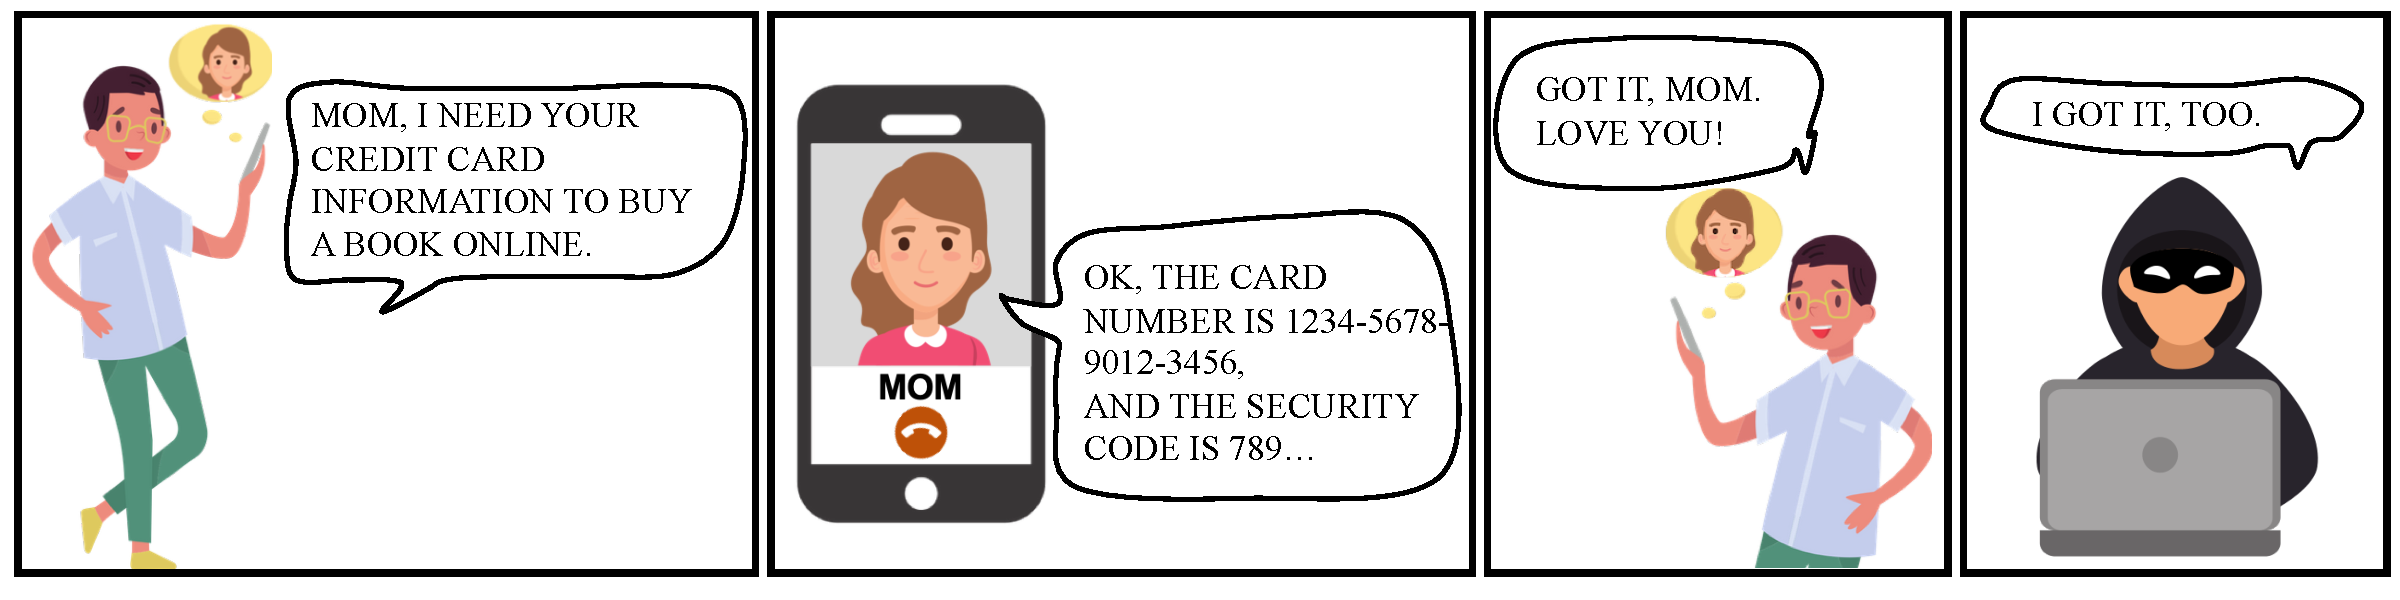
\includegraphics[width=\linewidth]{Figures/SpyPhone/teaserpic}
	\caption[Example of an Attacking Scenario.]{Example of an Attacking Scenario by {\spp}. A seemingly harmless application (a weather app for example) is installed on the phone, and it keeps accessing the motion sensors in background. Attackers can infer acoustic signals from the under-sampled motion data. }
	\label{fig:teaserpic}
\end{figure}



In fact, there have been some recent studies about the side-channel leakage from acoustic signals to smartphones' motion sensor readings. Michalevsky et al.~\cite{michalevsky2014gyrophone} proposed \textit{Gyrophone} in 2014. To the best of our knowledge, they are the first to use smartphone gyroscopes as low-frequency microphones to listen to loudspeakers. Gyrophone can differentiate 11 digits with 65\% accuracy based on a 10 people dataset.
%Michalevsky et al.~\cite{michalevsky2014gyrophone} are the first to use smartphone gyroscopes as low-frequency microphones. 
%However, they only tested their work on a small dataset (10 people) and achieved a digit recognition rate of 65\%. 
One year later, Zhang et al.~\cite{zhang2015accelword} proposed \textit{AccelWord}, which utilizes accelerometers to classify hotwords such as ``Okay Google'' or ``Hi Galaxy'' over other short phrases with 85\% accuracy. AccelWord is also tested over 10 people.
%However, their work lacks credibility due to limited dataset (10 people) and small classifying number (3 classes). 

However, techniques proposed in neither Gyrophone nor AccelWord can be used to perform a {\attackName} attack. Because these systems are built upon a \textit{speaker-dependent} model, i.e. training dataset are labeled data from the target speakers. In the {\attackName} attack, attackers will not get \textit{labeled} motion data from the victim  ------ the attack system should be \textit{speaker-independent}.

In 2018, Anald and Saxena~\cite{anand2018speechless} reproduced the aforementioned works and overturned their conclusions. They argued that smartphone motion sensors can not be affected by the speech signals transmitted through the air, no matter the sound source is a loudspeaker or a live person. They reported that only when the speakers and the motion sensors sharing a surface,  the \textit{conductive vibrations} will affect motion sensors' readings. Except for this ``Loudspeaker-Same-Surface'' scenario, they studied 5 other  scenarios
\footnote{\scriptsize``Loudspeaker-Different-Surface'', ``Laptop-Same-Surface'', `` Phone-Different-Surface'', 		``Human-Normal'', and ``Human-Loud''.}  
%(``Loudspeaker-Different-Surface'', ``Laptop-Same-Surface'', `` Phone-Different-Surface'', 		``Human-Normal'', and ``Human-Loud'')
and concluded that smartphone motion sensors only pose a limited threat to speech privacy.
% since conductive vibrations are ``possibly less common''.
%the impact of speech signals is very limited on motion sensors. 
%
However, they missed one important scenario,  the \textit{intra-device} scenario, where the speakers and motion sensors are inside the same smartphone. In 2019, they investigated this remaining scenario in an arXiv paper~\cite{anand2019spearphone} and their SpearPhone system recognize 11 digits with an accuracy of 71\%.  However, their technique is still speaker-dependent, which means the original speech data of the target speaker must be collected ahead of time. Such requirement is very hard to be fulfilled in practice.

In this thesis, we studied the side-channel attack in the intra-device scenario. This \textit{{\attackName}} attack, as we refer to it, is speaker-independent.


%\begin{figure}[!h]
%\centering
%\subfloat[][]{.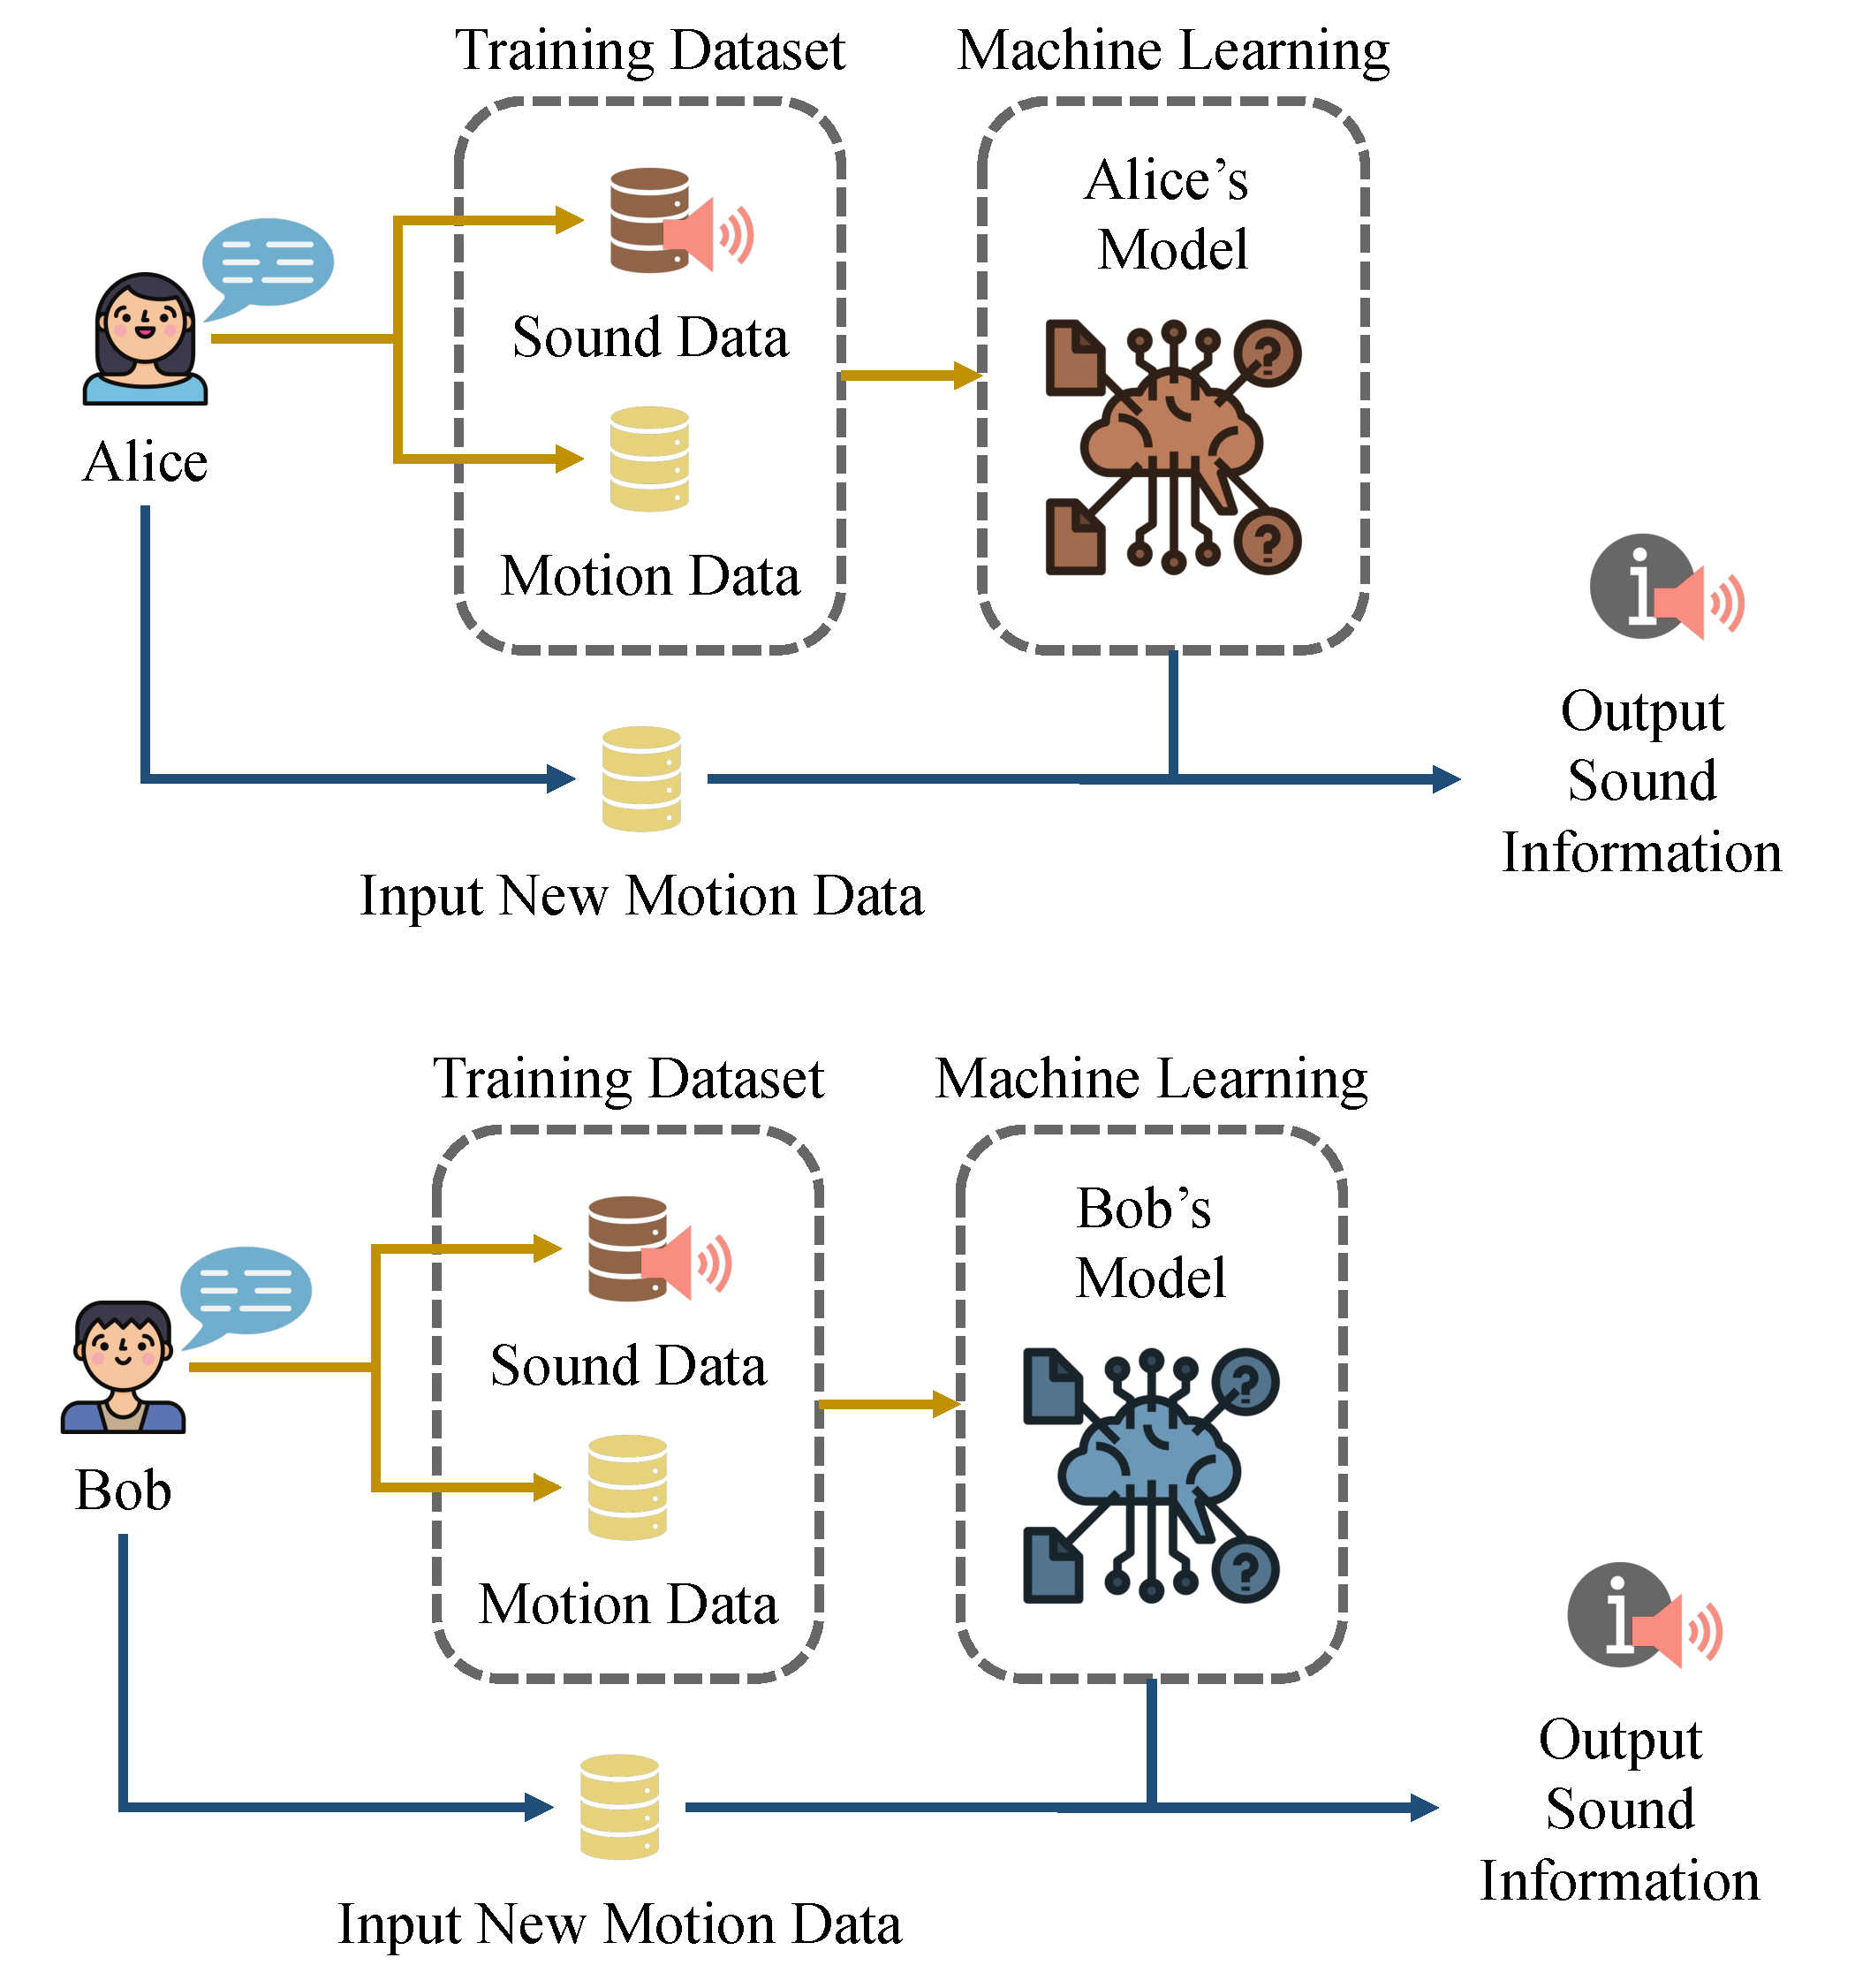
\includegraphics[width=.9\linewidth]{speakerDependent}
%	\vspace{-.05in}
%	\caption{Mathematical model of a typical compressed sensing system. }%
%\qquad
%\subfloat[][]{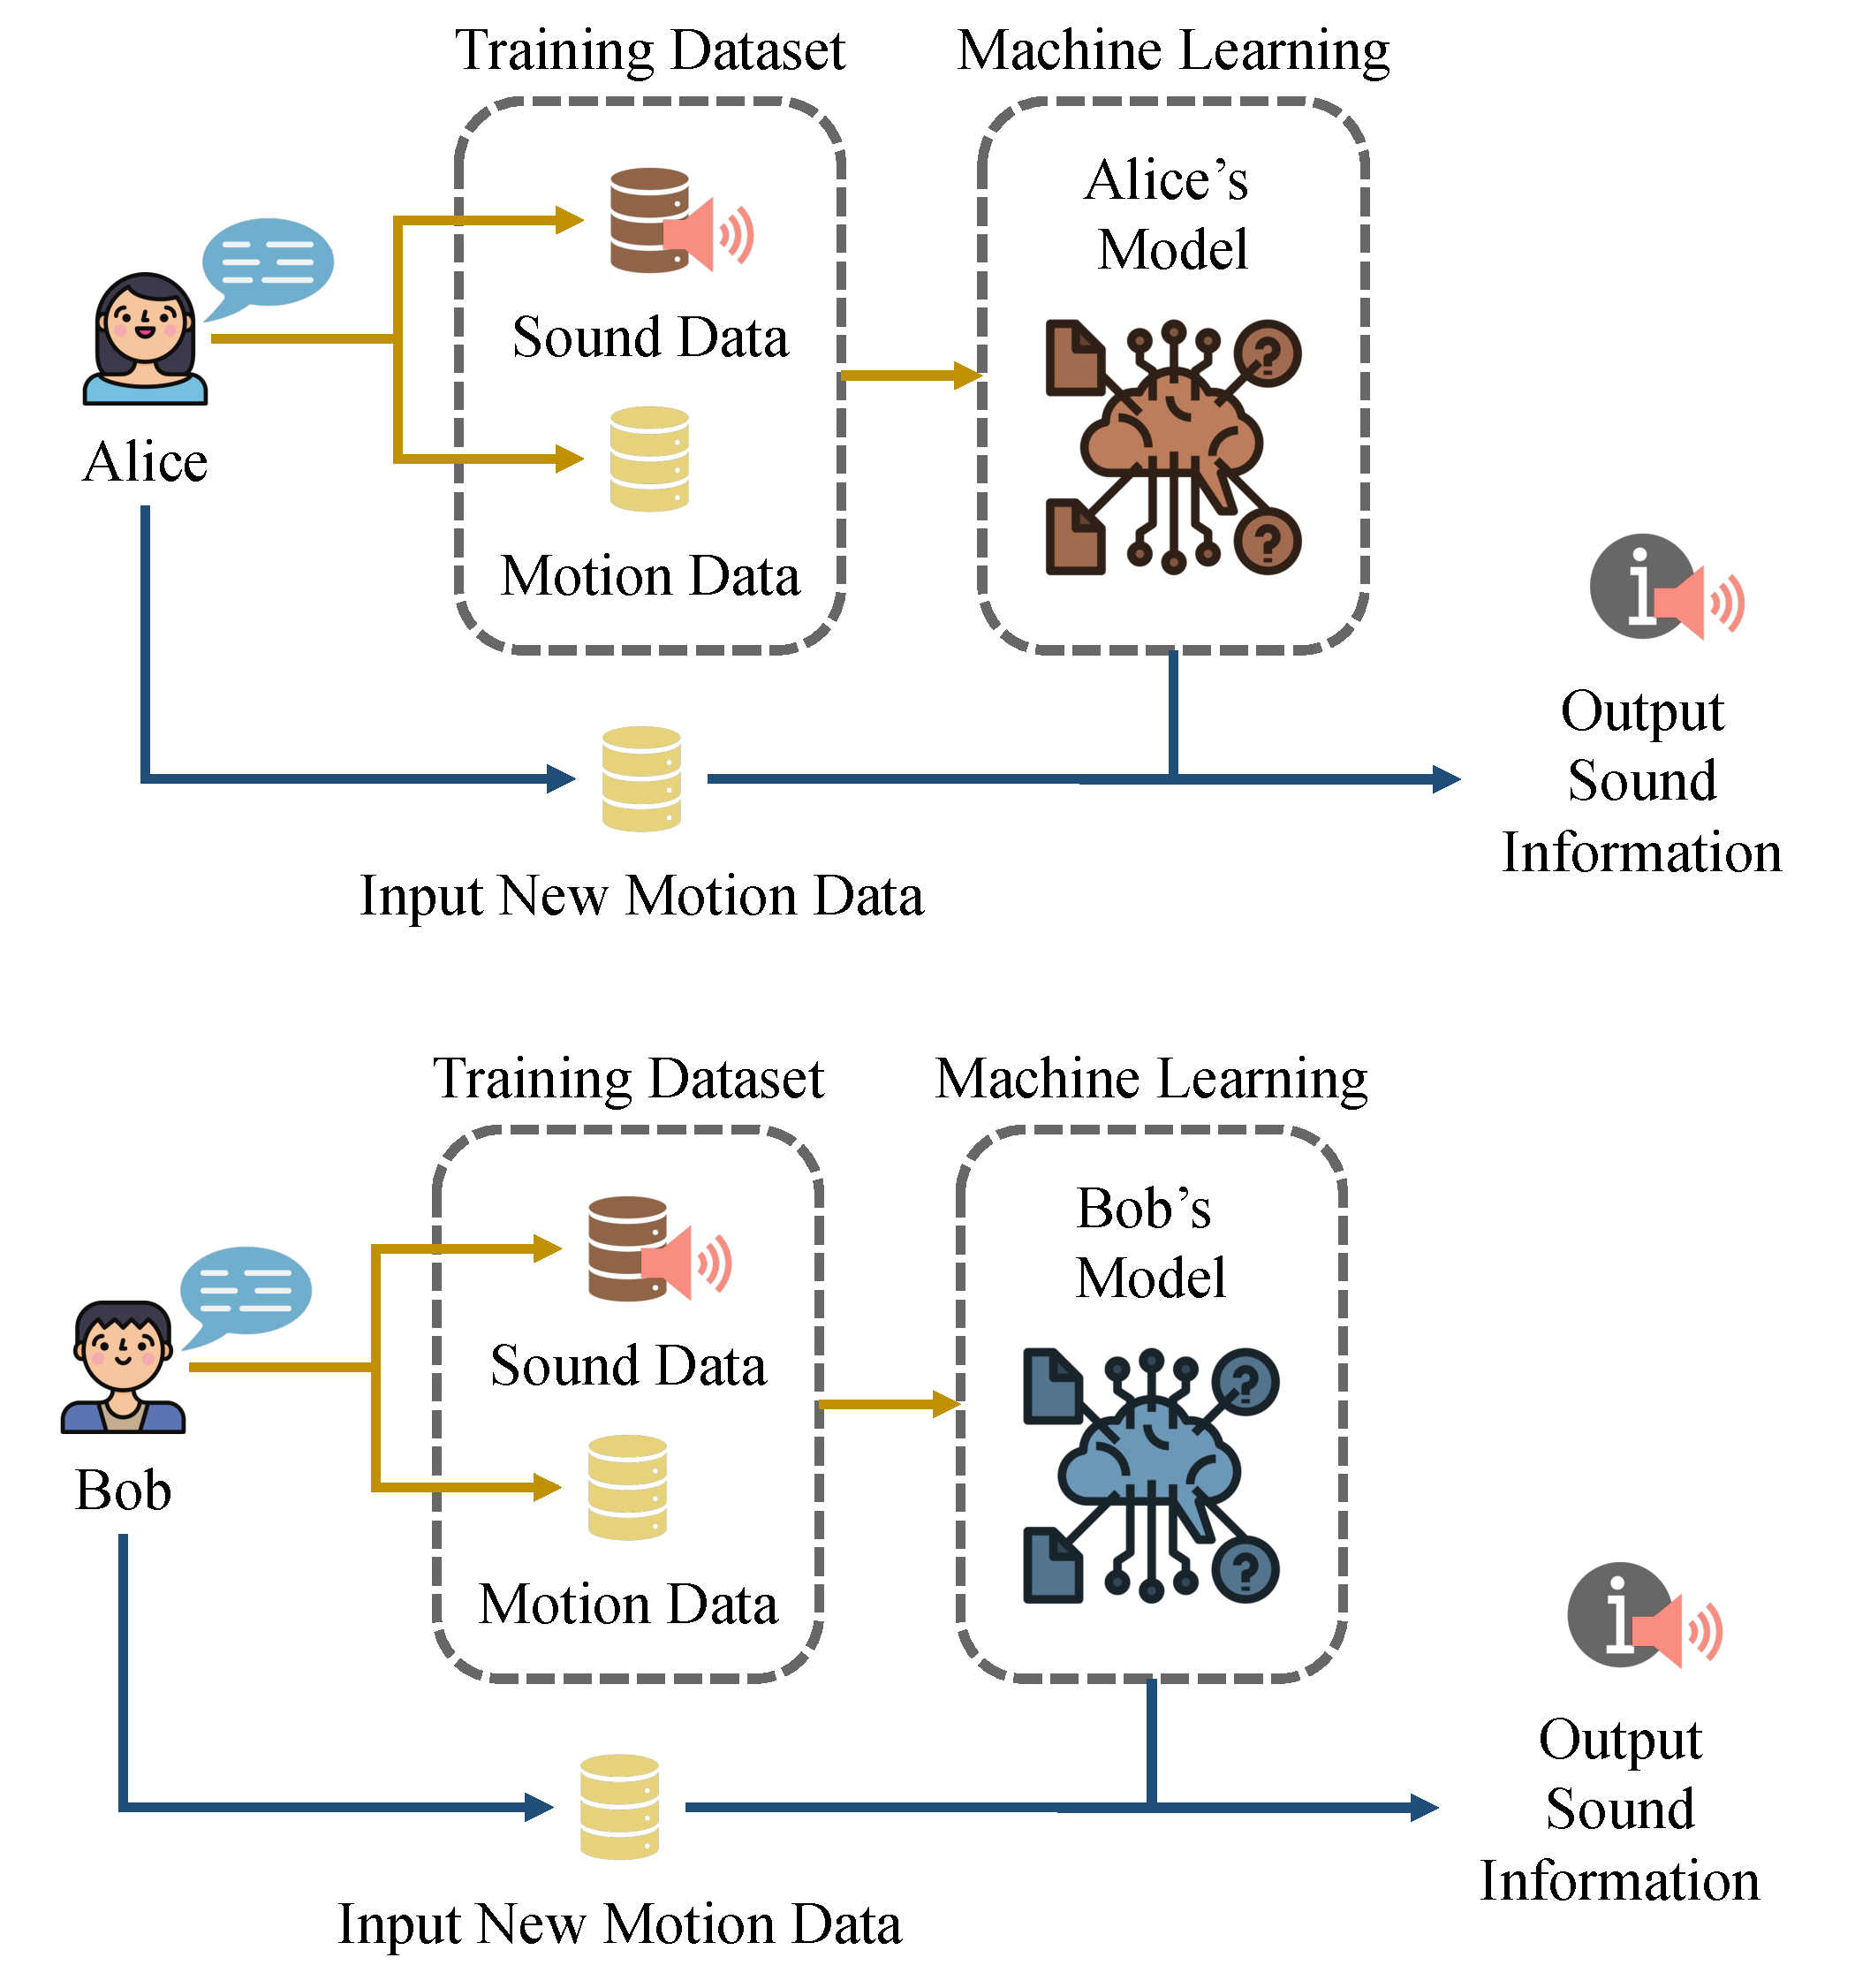
\includegraphics[width=.9\linewidth]{speakerDependent}
%	\vspace{-.05in}
%	\caption{Mathematical model of a typical compressed sensing system. }
%\caption{Here are the first two figures of a continued figure.}% \label{fig:cont}
%\end{figure}
% Attackers do not need to get the target victim's speech data and they can still filch critical information from the 


% https://arxiv.org/abs/1907.05972
%The side-channel attack in this scenario, or the \textit{{\attackName}} attack as we refer to it, is the focus of this paper. We agree with Anald and Saxena on that motion sensors are more sensitive to conductive vibrations than aerial vibrations, but we show motion sensors can leak various critical information and pose a big threat to smartphone users' security and privacy. 

% accelerometer when the laptop and the motion sensor shared a surface.
%
%direct acoustic aerial vibrations 
%
%
%aerial vibrations. We also report that in the presence of live human speech, we did not 
%
% the recorded effect on the sensor readings is possibly from conductive vibrations through the shared surface instead of direct acoustic vibrations due to speech as perceived in previous work. S
%
%
%. They stated that smartphone speakers were not found to be powerful enough to invoke a response in the motion sensors \textit{through aerial vibrations}. They also reported that in the presence of live human speech, they did not notice any effect on the motion sensor readings.

%Different research groups draw conflicting conclusions. So who is right? We have done similar experiments and the findings are similar to that of Anald and Saxena. Unless a person speaks really loudly (shouting, usually 10 dB higher than normal speech),  or use commercial loudspeakers (not MEMS speakers inside smartphones) on the same surface with the smartphone, it is hard to identify the sounding period based on motion sensors. Moreover, the distance between the sound source and the smartphones must be short (less than 30 cm). 

%However, Anald and Saxena's work is not perfect. Although they studied this side-channel leakage in 6 different scenarios and showed the threats only have significant impacts in the ``Loudspeaker-Same-Surface'' scenario, they missed one important scenario, the \textit{intra-device} case, where the speakers and motion sensors are inside the same device. This scenario, or the \textit{{\attackName}} attack as we refer to it, is the focus of our research.

%
%It is also worth mentioning that prior works such as  Gyrophone~\cite{michalevsky2014gyrophone} and AccelWord~\cite{zhang2015accelword} can only achieve the claimed accuracy in the speaker-dependent setting. But a speaker-dependent setting requires the system to get specific training data from the target user. Such condition may not be satisfied in real attacking scenarios. When Gyrophone use an speaker-independent setting to identify digits, the maximum accuracy  is only 26\%.

\begin{table}[h]
	\caption{Maximum Sampling Rate of Smartphone Sensors}
	%	\footnote{Some part of the data is from~\cite{matyunin2018zero}, others are tested }
	\label{tab:sample}
	\centering
	
	%	\resizebox{\columnwidth}{!}{
	\begin{tabular}{cccc} %{lp{2cm}p{2cm}}
		\toprule		
		Device & \makecell{Release \\Year} & \makecell{Speakers' \\ Sampling Rate} & \makecell{Motion Sensors' \\ Sampling Rate
			\footnotemark} \\
		\midrule
		Samsung Galaxy S8 & 2017 & 192,000 Hz & 500 Hz\\
		Samsung Galaxy S7 & 2016 & 192,000 Hz & 500 Hz\\		
		Google Nexus 6P & 2015 & 48,000 Hz & 400 Hz\\
		LG Nexus 4 & 2012 & 48,000 Hz& 200 Hz\\
		\bottomrule
	\end{tabular}
	%}
\end{table}



\footnotetext{\scriptsize Data is partially from~\cite{matyunin2018zero} and partially by calling the \texttt{getMinDelay()} function of \texttt{android.hardware.Sensor} class.}

%To sum up, we show how to design an eavesdropping system that measures the conductive vibrations from smartphones' built-in MEMS speakers to MEMS accelerometers and gyroscopes. The main challenges in performing such an attack are:
%In this paper, we design an eavesdropping system named \textit{{\systemName}} which implements the speaker-independent {\attackName} attack. 
The main challenges in designing such a system are:
 \begin{itemize}
 	\item  The motion sensor readings are affected by at least four types of signal sources: sensor intrinsic errors, movement of the smartphone, acoustic vibrations from built-in speakers, acoustic vibrations from the air or other sound sources. An efficient filter is needed since only the acoustic vibrations from built-in speakers is the signal of interest.
 	
 	\item As shown in Table~\ref{tab:sample}, compared to the sampling rate of smartphones' built-in speakers which can reach 192 kHz, the sampling rate of motion sensors is 200-500 Hz. With such low frequency, human ears are no longer able to retrieve the original information, neither do state-of-the-art speech recognition systems~\cite{michalevsky2014gyrophone}.
 	
 	\item As illustrated in Figure~\ref{fig:depend}, the system should be speaker-independent. Prior works such as  Gyrophone~\cite{michalevsky2014gyrophone} and AccelWord~\cite{zhang2015accelword} can only achieve the claimed accuracy (65\% for 11 classes and 85\% for 3 classes) in the speaker-dependent setting. When Gyrophone uses an speaker-independent setting to identify digits, the
 	accuracy is only 26\%. This indicates that building a speaker-independent system is much more challenging than a speaker-dependent one.
 	
% 	harder than a speaker-dependent system.
% 	%TODO.
% 	In addition
% 	However, the speaker-dependent setting requires the system to get specific training data from the target user. Such condition may not be satisfied in real attacking scenarios. 
 \end{itemize}

%
%44.1 kHZ, 48kHz, 96kHz, or even 192kHz\footnote{Example sampling rate as shown in \url{https://developer.android.com/ndk/guides/audio/sampling-audio}.}, 
%The impact of the studied threat under the designed scenarios therefore limits itself to only specific settings. F
%
%
%information leakage from physical properties, or side-channels


%
%Consequences:
%know the gender
%know the number
%know your activity
%
%Contributions
%

%How we conquer the challenges?

%Although reconstructing original sound signals from motion data is impossible, partial information can be learned by {\attackName} attackers. Such information includes user activity, speaker gender/identity, and speech content (as elaborated in Section~\ref{sec:threat}). 

%\footnote{We refer the attack as the {\attackName} attack, and the system designed to perform such an attack as the {\systemName} system.}



Despite these challenges, the {\systemName} system is able to learn variety of critical information from smartphone users, such as user activity, speaker gender/identity, and speech content (as elaborated in Section~\ref{sec:threat}). 
These achievements are largely credited to the compressed sensing theories which allow recovering certain signals from fewer samples than required in Nyquist paradigm (as elaborated in Section~\ref{sec:background}); and the machine learning techniques named Bi-directional Long Short-Term Memory (Bi-LSTM) network, which is a special variant of recurrent neural networks. 




\begin{landscape}
	\begin{figure*}[h]%
		\centering
		\begin{minipage}[c]{.45\linewidth}
%			\begin{subfigure}[t]{1.3\textwidth}
				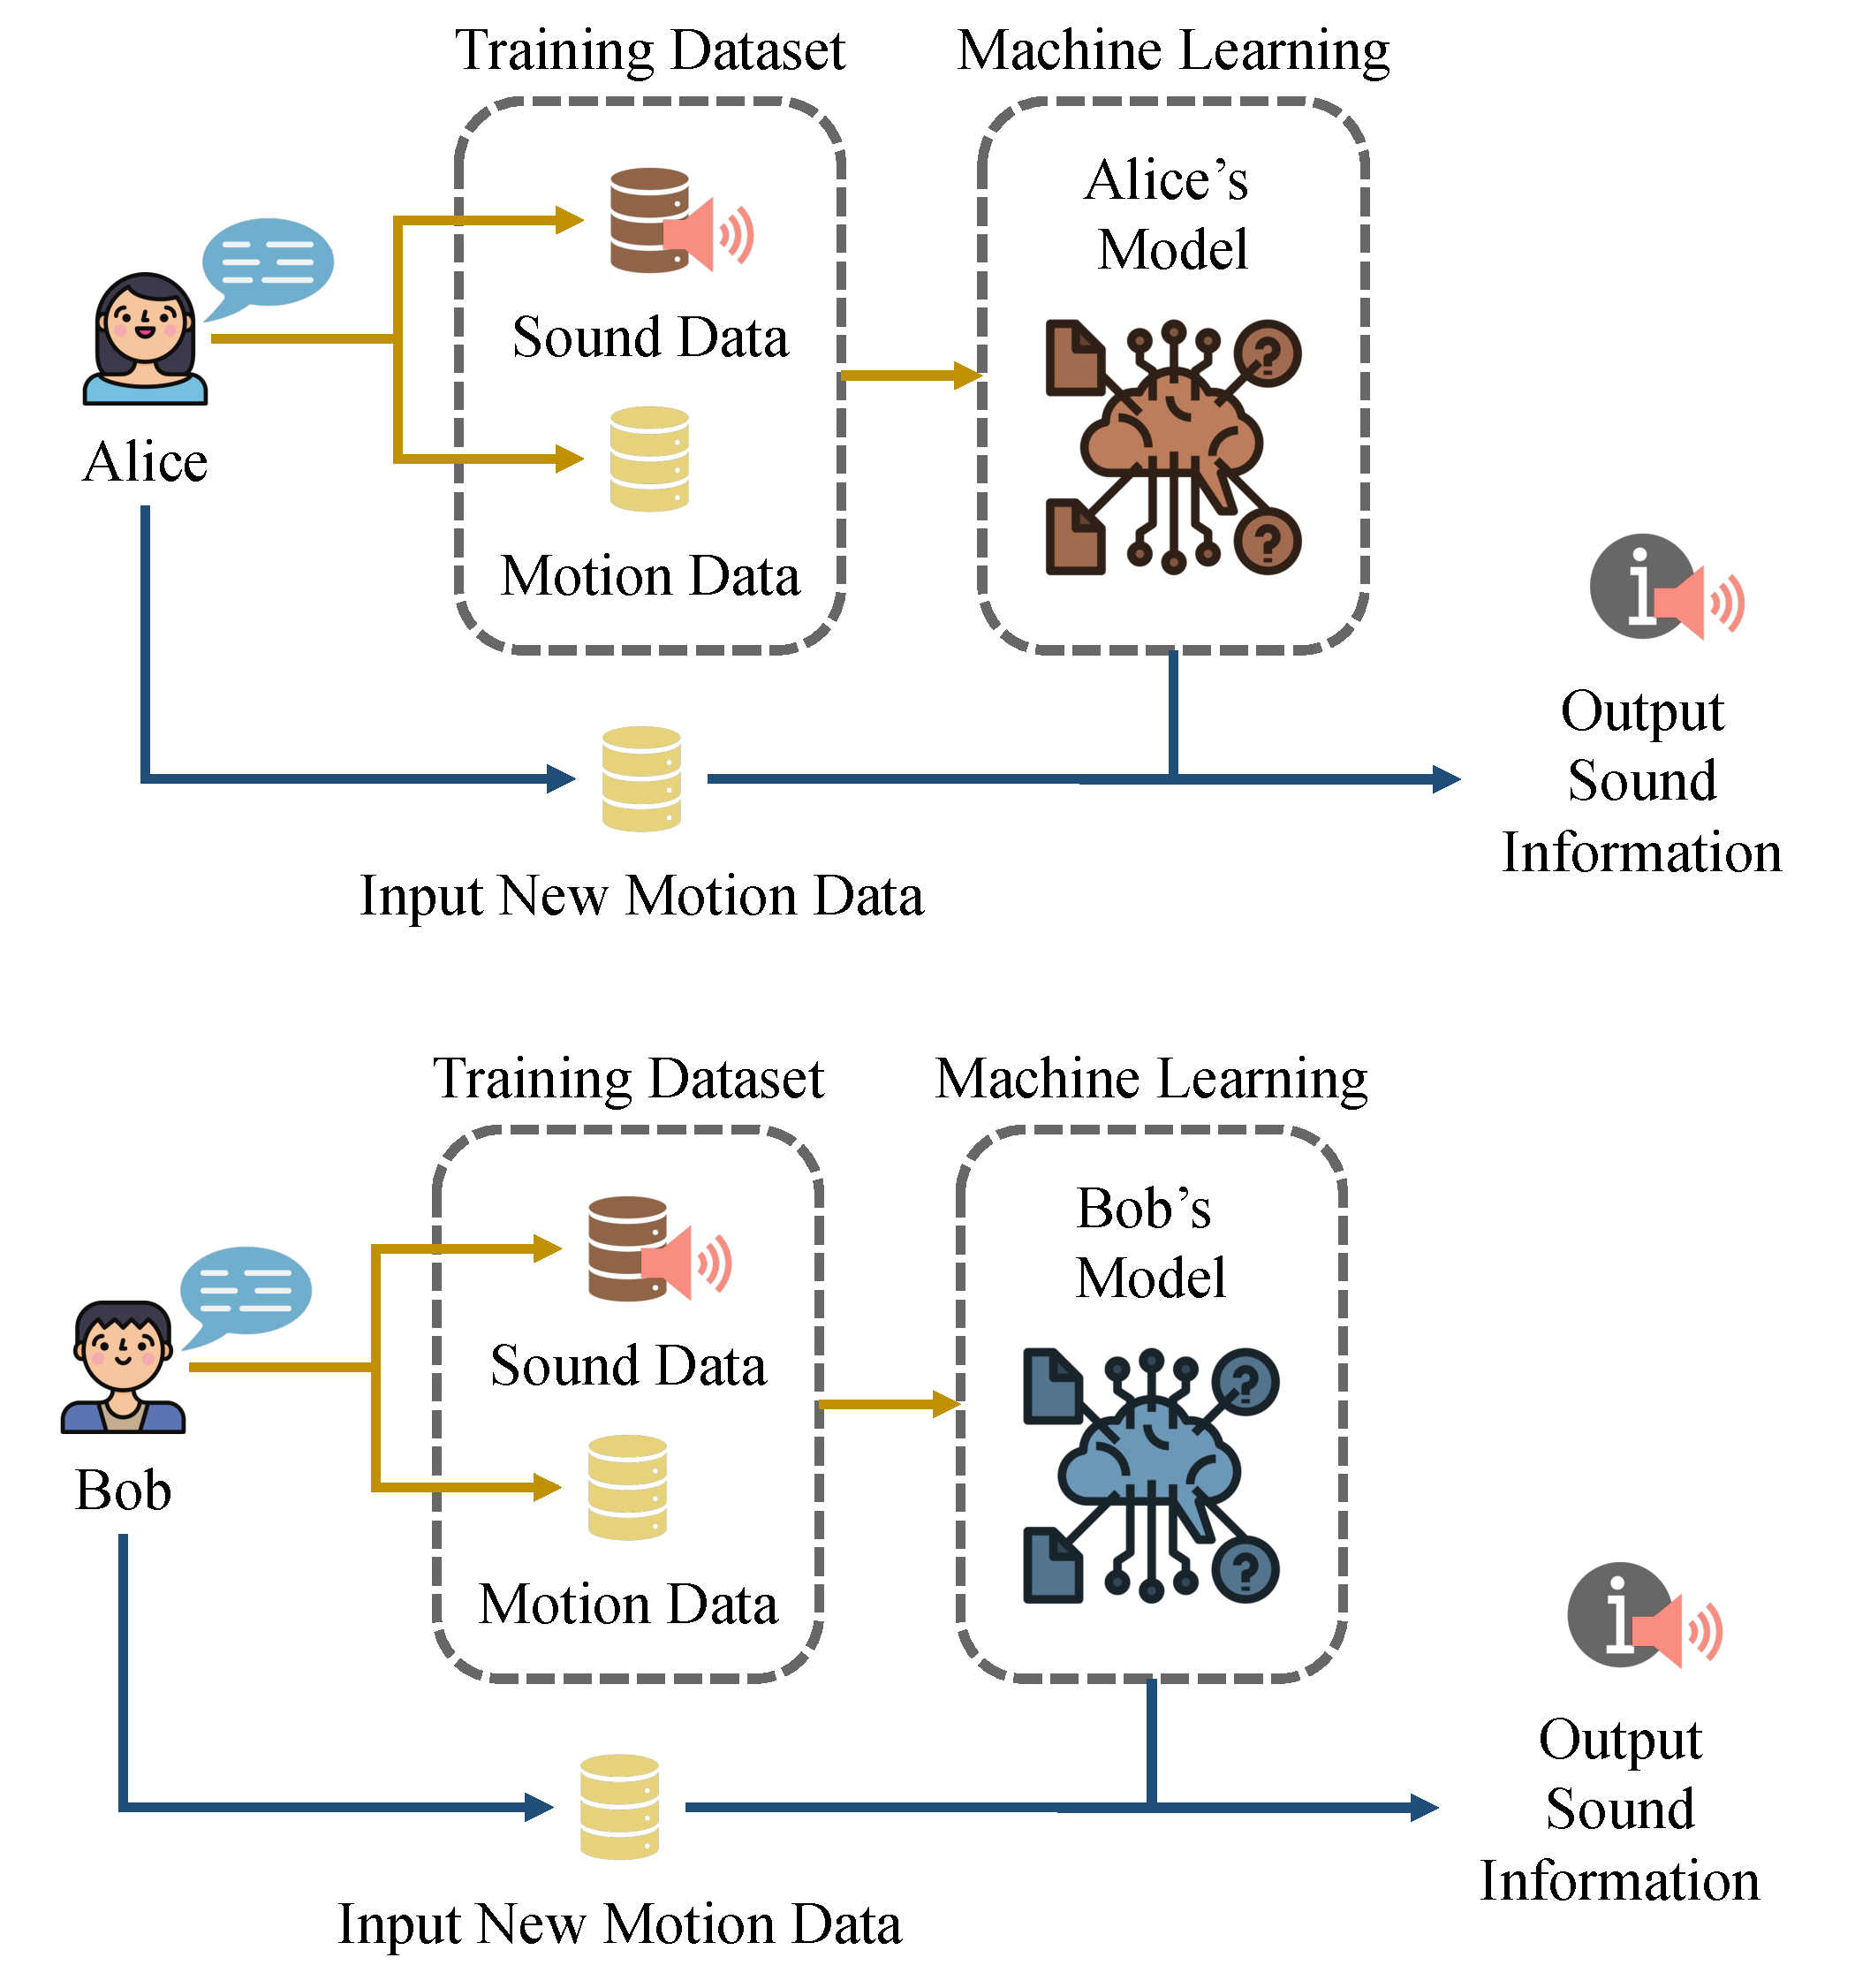
\includegraphics[width=\textwidth]{speakerDependent}
				\subcaption{Speaker-Dependent: target speaker's training data is required. After machine learning procedures, the trained models  for different speakers are different.}
%			\end{subfigure}
		\end{minipage}
		\begin{minipage}[t]{.05\textwidth}
			\qquad
		\end{minipage}
		\begin{minipage}[c]{.45\linewidth}
%			\begin{subfigure}[t]{1.25\textwidth}
				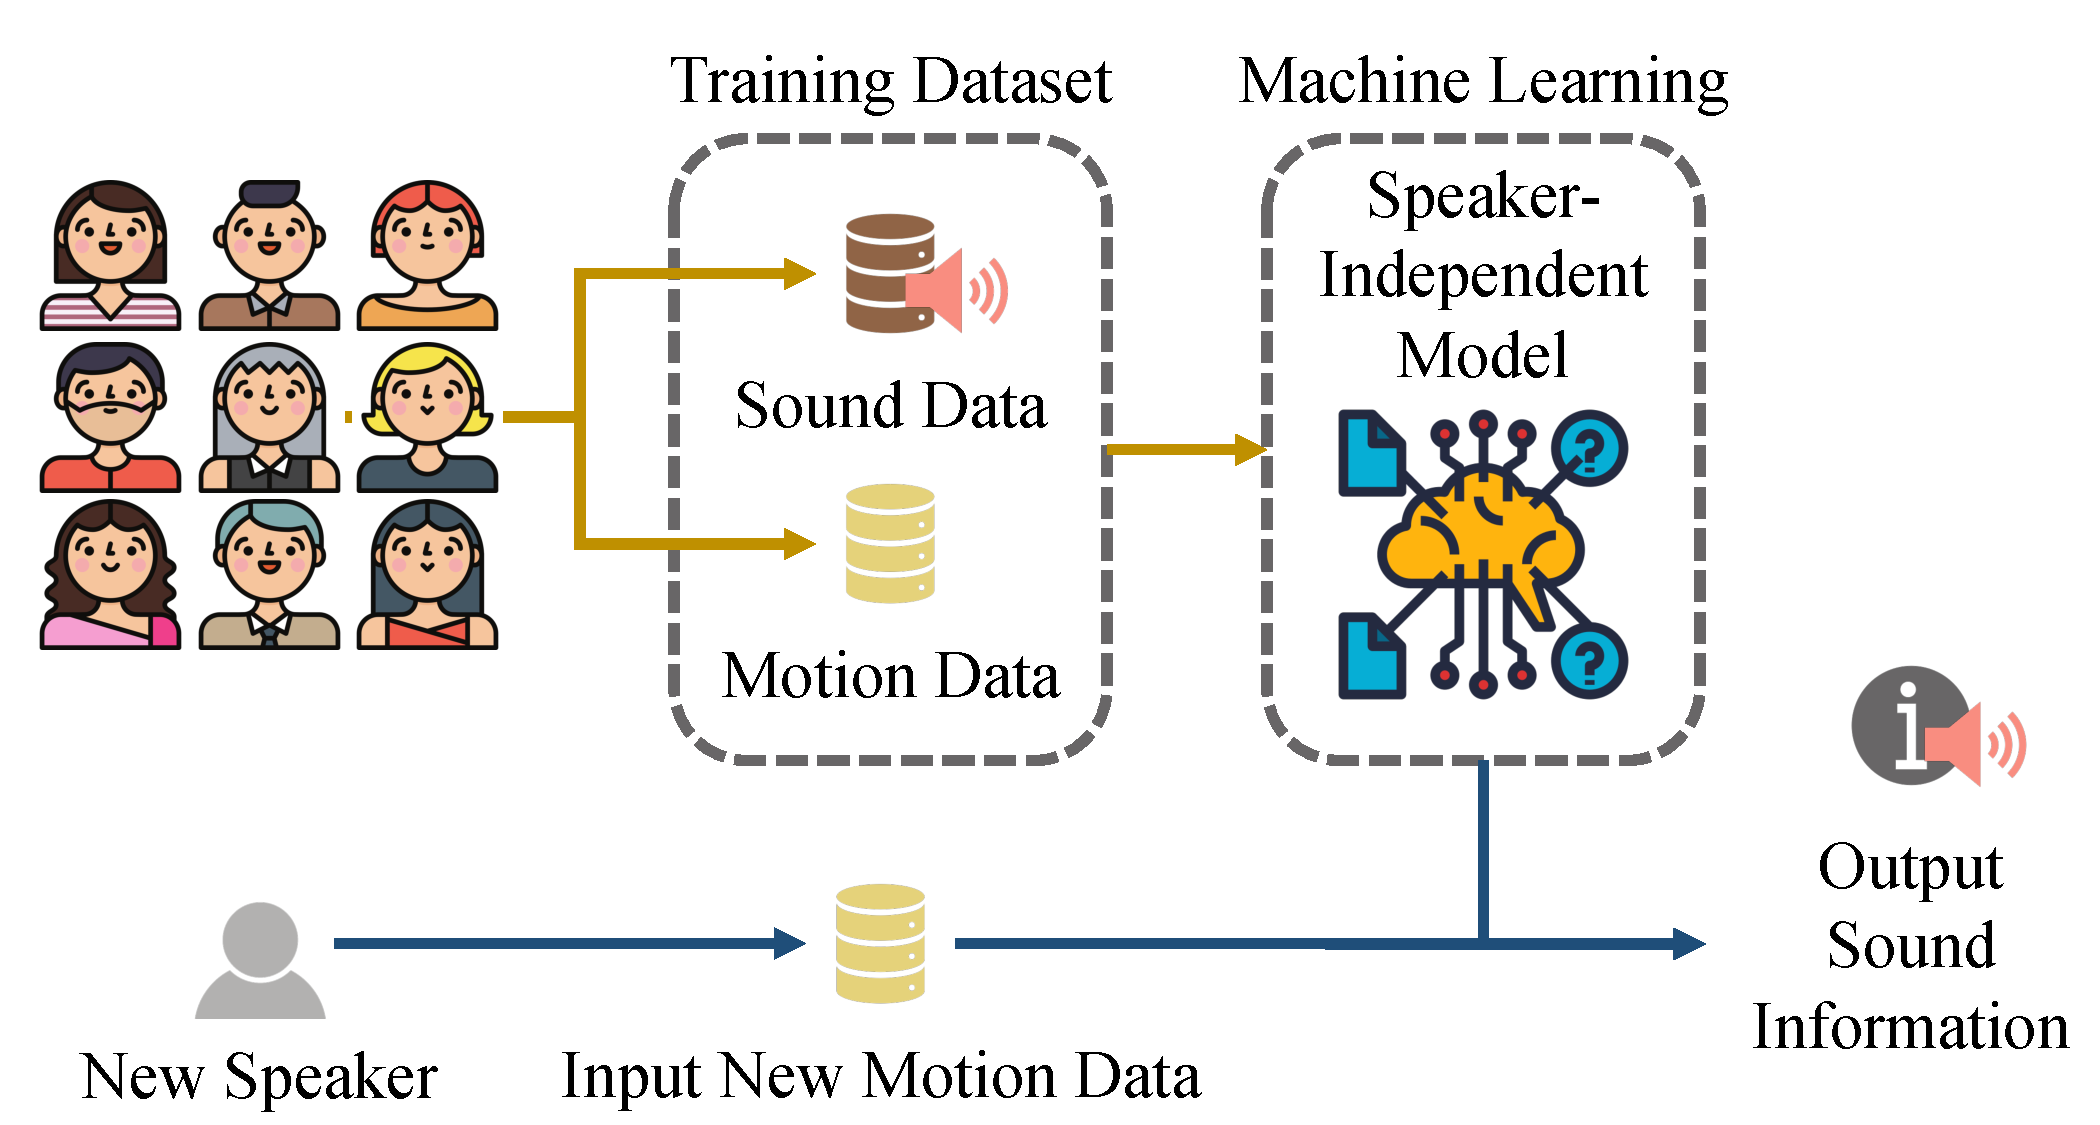
\includegraphics[width=\textwidth]{speakerIndependent}
				\subcaption{Speaker-Independent: the model is trained on a group of speakers, and can be used to predict brand new speakers.}
%			\end{subfigure}
		\end{minipage}
		\caption{{\attackName} Attack Should be Speaker-Independent.} \label{fig:depend}
	\end{figure*}
\end{landscape}

%We conquer the challenges by various  signal processing techniques 

%In summary, our contributions are listed as follows.
%This dissertation offers the following contributions:
%The main contributions are summarized as follows:
%
In summary, our main contributions are as follows:
\begin{itemize}
	\item 
	We uncover a new stealth attack named the {\attackName} attack that eavesdrops on smartphones' built-in speakers by the intra-device motion sensors. Existing techniques in Gyrophone~\cite{michalevsky2014gyrophone} and AccelWord~\cite{zhang2015accelword} cannot be used for the {\attackName}  attack because their system are speaker-dependent, which require the training speech data from the victim. The {\attackName}  attack, however, removes this requirement and thus is more dangerous and harmful.
	
	\item 
	To the best of our knowledge, we are the first to apply compressed sensing theories in the audio-to-motion side-channel data so as to bridge the gap between sampling rates. This is the core technique we used to achieve speaker-independent of the attacking system.
	
	
	\item 
	We design the {\systemName} system and validate its feasibility on learning user activity, speaker gender/identity, and speech content.  {\systemName} system can achieve higher accuracy than existing works. In addition, we have studied how different internal parameters (used in algorithms) and external parameters (properties of input data) affect the  performance of this system.
	
	
%	\item User-independent no individual training
%	
%	Unnoticeable, universal
\end{itemize}


















%%%%%%%%%%%%%%Materials%%%%%%%%%%%%%%



%~\cite{aaaGoogleSearch,michalevsky2014gyrophone,matyunin2018zero}

%
%Any app installed on a smartphone  is permitted to access to motion sensors 


%the system automatically grants the app that permission at install time. 
%%TODO side channal attack??

 
%Why can smartphones provide so many efficient and user-friendly applications? Because these smart devices seamlessly integrate the physical world with the cyber world via their sensors (e.g., light, accelerometer, gyroscope, microphone, speaker, camera, GPS, etc.)~\cite{sikder20176thsense}.
%
%
%
%However, the presence of sensors also has the dark side: \textit{sensor-based attack}s on smartphones. 
%
%The feasibility of keystroke inference from nearby key- boards using accelerometers has been shown in [35]. In [21], the authors demonstrate the possibility of keystroke inference on a mobile device using accelerometers and mention the potential of using gyroscope measurements as well, while another study [19] points to the benefits of exploiting the gyroscope.
%While the number of applications using different sen- sors [38] is increasing and new devices offer more sen- sors, the presence of sensors have opened novel ways to exploit the smart devices [76]. Attackers can exploit the sensors in many different ways [76]: they can trig- ger an existing malware on a device with a simple flash- light [28]; they can use a sensor (e.g., light sensor) to leak sensitive information; using motion sensors such as ac- celerometer, and gyroscope, attackers can record or steal sensitive information from other nearby devices (e.g., computers, keyboards) or people [10, 87, 26, 42]. They can even transfer a specific malware using sensors as a communication channel [76]. Such sensor-based threats become more serious with the rapid growth of Apps uti- lizing many sensors [6, 2].
%
%
%In fact, these sensor-based threats highlight the flaws of existing sensor management systems used by smart devices. Specifically, Android sensor management sys- tem relies on permission-based access control, which considers only a few sensors (i.e., microphone, camera, and GPS)1. Android asks for access permission (i.e., with a list of permissions) only while an App is being installed for the first time. Once this permission is granted, the user has no control over how the listed sensors and other sensors (not listed) will be used by the specific App. Moreover, using some sensors is not considered as a vi- olation of security and privacy in Android. For instance, any App is permitted to access to motion sensors by just accessing the sensor API. Access to motion sensors is not controlled in Android.


%Android sensor management
%
%In this paper, we show how to use only motion sensors to eavesdrop on everything played by the smartphones' built-in speakers, i.e., how to turn the existing over 3 billion smartphones to billions of spy-phones.
%
%This attack is based on the fact that...


%Four  papers: Gyrophone, WALNUT, AccelWord, Speechless
%
%
%
%spy bugs and listening devices
%
%Smartphones are everywhere. 
%
%
%
%
%Existing Eavesdropping on smartphones
%
%Prior work like gyrophone and accelword


% Smartphones are everywhere.
%
%versatile handheld devices have become indispensable tools,
%
%Generally, older "feature" phones are capable of voice calls, text messages and the occasional photo, but not much else. Smart phones, on the other hand, are essentially handheld computers. Users can check their email, browse the web, post updates to social media sites, play games, listen to music, watch movies and even shoot video.
%
%The capabilities are so extensive, 
%
%
%From teenagers to seniors, people 
%
%
%However, the ubiquity of smartphones not only bring convenience to legitimate users, but also build a hotbed of new types of attacks.
%
%According to reports issued by several market-research firms,  including Forrester Research, the total number of smartphone users worldwide will reach 3 billion this year—40 percent of the human population. 
%
%Who doesn’t own a Smartphone? Right from teenagers to senior citizens and from businesspersons to business leaders, Smartphone ownership is Ubiquitous and all pervasive. Indeed, it is estimated that nearly 80\% of the world’s population is now connected to each other through the mobile phones with Smartphones constituting the majority of such devices.
%
%
%
%THE dawn of the planet of the smartphones came in January 2007, when Steve ... The smartphone is ubiquitous, addictive and transformative .
%
%
%The Smartphone is everywhere. Its Ubiquity has resulted in new forms of capitalism with Entrepreneurs and Traders using it for direct communication and  ...
%
%
%According to reports issued by several market-research firms, including Forrester Research, the total number of smartphone users worldwide will reach 3 billion this year—40 percent of the human population. For many, these versatile handheld devices have become indispensable tools, providing connections to loved ones, entertainment, business applications, shopping opportunities, windows into the greater world of social media, news, history, education, and more. And of course, they can always be put to use for a quick selfie. With so many devices in so many hands now, the visual landscape has changed greatly, making it a rare event to find oneself in a group of people anywhere in the world and not see at least one of them using a phone. Collected here: a look at that smartphone landscape, and some of the stories of the phones’ owners.
